\documentclass[11pt, a4paper]{book}
\usepackage{parskip}
\usepackage[top=1.5cm, left=1cm, right=1cm, bottom=2.5cm]{geometry}
\usepackage{fontspec}
\usepackage{graphicx}
\setmainfont{DejaVu Serif}

\begin{document}
\chapter{Lexi Use case summary}
\begin{description}
\item [Composite] To represent the document's \emph{physical structure}
\item [Strategy] To allow different formatting algorithm.
\item [Decorator] For embellishing the user interface
\item [Abstract Factory] For supporting multiple look-and-feel.  \item [Bridge] To allow multiple windowing platforms
\item [Command] For undoable user operations.
\item [Iterator] For accessing and traversing object structures
\item [Visitor] For allowing an open-ended number of analytical capabilities
without complicating the document structure's implementation.
\end{description}

\chapter{Creational Design Pattern}
Creational design patterns \textbf{abstract the instantiation process}. They
help make a system \emph{independent of how its objects are created, composed,
and represented}. A class creational pattern uses inheritance to vary the class
that's instantiated, whereas an object creational pattern will delegate
instantiation to another object.

Tow recurring themes in these patters:
\begin{enumerate}
    \item They all encapsulate knowledge about which concrete classes the system
    uses.
    \item They hide how instances of these classes are created and put together.
\end{enumerate}
Consequently, the creational patterns give you a lot of flexibility in
\emph{what} gets created, \emph{who} gets creates it, \emph{how} it cets
created, and \emph{when}.

They let you configure a system with "product" objects that very widely in
structure and functionality. See the MaseExample.cpp.

Refer to the MaseExample:
\begin{description}
    \item [Factory Method] If CreateMaze calls \emph{virtual functions} instead of constructor
    calls to create the rooms, then you can change the classes that get
    instantiated by making a subclass of MazeGame and redefining those virtual
    functions
    \item [Abstract Factory]If CreateMaze is passed an object as a parameter to use to create
    rooms, walls and doors, then you can change the classes of rooms, walls, and
    doors by passing a different parameter.
    \item [Builder] If CreateMaze is passed an object that can create a new maze
    in its entirety using operations for adding rooms, doors, and walls to the
    maze it builds, then you can use inheritance to change parts of the maze or
    the way the maze is built.
    \item [Prototype] If CreateMaze is parameterize by various prototypical
    room, door, and wall objects, which it then copies and adds to the maze,
    then you can change the maze's composition by replacing these prototypical
    objects with different ones.
    \item [Singleton] Ensure there's only one mazze per game and that all game
    objects have ready access to it.
\end{description}

\section{Abstract Factory}
\subsection{Intent}
Provide an interface for creating \emph{families of related or dependent
objects} without specifying their concrete classes. Also known as kit.
\subsection{Motivation}
Widgets that can have different look-and-feel. An application should not
hard-code its widgets for a particular look an dfeel.

Solve this problem by defining an abstract \verb|WidgetFactory| class that
declares an interface for reating each basic kind of widget.

There's also an abstract class for each kind of widget, and concree subclasses
implement widgets for specific look-and-feel.

WidgetFactory's interface has an operation that returns a new widget object for
each abstract widget class. Clients call these operations to obtain widget
instances, \emph{but clients aren't aware of the concrete classes they're
using.} Thus clients stay independent of the prevailing look and feel.

There is a concrete subclass of WidgetFactory for each look-and-feel.
\subsection{Applicability}
Use Abstract Factory when:
\begin{itemize}
    \item A system should be independent of how its products are created,
    composed, and represented.
    \item A system should be configured with one of multiple families of
    products.
    \item A family of related product objects is designed to be used together,
    and you should enforce this constraint.
    \item You want to provide a class library of products, and you want to
    reveal just their interfaces, not their implementations.
\end{itemize}
\subsection{Participants}
\begin{description}
    \item [AbstractFactory] declares an interface for creating operation
    \item [ConcreteFactory] implement the interface to create concrete product.
    \item [AbstractProduct] declares an interface for a type of product.
    \item [ConcreteProduct] Defines a product object to be created by the
    corresponding concrete factory. Implements interfaces of AbstractProduct.
    \item [Client] Uses only interfaces declared by AbstractProduct and
    AbstractFactory classes.
\end{description}
\subsection{Consequence}
\begin{enumerate}
    \item It isolates concrete classes.
    \item It makes exchanging product families easy.
    \item It promotes consistency among products.
    \item Supporting new kinds of product is difficult. That's because the
    AbstractFactory interface fixes the set of products that can be created
\end{enumerate}
\subsection{Implementation}
Some useful techniques for implementing the Abstract Factory Patter:
\begin{enumerate}
    \item Factories as singletons.
    \item Creating the products. The most common way to do this is to define a
    factory method for each product. If many product families are possible, the
    concrete factory can be implemented using he \textbf{Prototype} pattern. The
    concrete factory is initialized with a prototypical instance of each product
    in the family, and it creates a new product by cloning its prototype.
    \item Defining extensible factories. Add a parameter to operations that
    create objects. This parameter specifies the kind of object to be created.
    It could be a class identifier, a string or anything else that identifies
    the kind of product. This variation is easier to use in dynamically typed
    language like Smalltalk than in a statically typed language like C++. You
    can use it in C++ only when all objects have the same abstract base class or
    when the product objects can be safely coerced to correct type by the
    client that requested them.
\end{enumerate}
\subsection{Sample Code}
Class \verb|MazeFactory| can crete components of mazes.
\begin{verbatim}
class MazeFactory {
public:
    MazeFactory();
    virtual Maze* MakeMaze() const
        { return new Maze; }
    virtual Wall* MakeWall() const
        { return new Wall; }
    virtual Room* MakeRoom(int n) const
        { return new Room(n); }
    virtual Door* MakeDoor(Room* r1, Room* r2) const
        { return new Door(r1, r2); }
};
\end{verbatim}
Here's a version that taking a \verb|MazeFactory| as a parameter:
\begin{verbatim}
Maze* MazeGame::CreateMaze (MazeFactory& factory) {
    Maze* aMaze = factory.MakeMaze();
    Room* r1 = factory.MakeRoom(1);
    Room* r2 = factory.MakeRoom(2);
    Door* aDoor = factory.MakeDoor(r1, r2);

    aMaze->AddRoom(r1);
    aMaze->AddRoom(r2);

    r1->SetSide(North, factory.MakeWall());
    r1->SetSide(East, aDoor);
    r1->SetSide(South, factory.MakeWall());
    r1->SetSide(West, factory.MakeWall());

    r2->SetSide(North, factory.MakeWall());
    r2->SetSide(East, factory.MakeWall());
    r2->SetSide(South, factory.MakeWall());
    r2->SetSide(West, aDoor);

    return aMaze;
}
\end{verbatim}
We can create \verb|EnchantedMazeFactory|, a factory for enchanted mazes, by
sublcassing \verb|MazeFactory|.
\begin{verbatim}
class EnchantedMazeFactory : public MazeFactory {
public:
    EnchantedMazeFactory();

    virtual Room* MakeRoom(int n)  const
        { return new EnchantedRoom(n, CastSpell()); }

    virtual Door* MakeDoor(Room* r1, Room* r2)  const
        { return new DoorNeedingSpell(r1, r2); }

protected:
    Spell* CastSpell() const;
};
\end{verbatim}

Another class of \verb|BombedMazeFactory| a subclass of \verb|mazeFactory|.
BombedMazeFactory only needs to override two functions:
\begin{verbatim}
Wall* BombedMazeFactory::MakeWall() {
    return new BombedWall;
}
Room* BombedMazeFactory::MakeRoom(int n) {
    return new RoomWIthABomb(n);
}
\end{verbatim}
To build a simple maze that can contain bombs, we simple call \verb|CreateMaze|
wth a \verb|BombedMazeFactory|:
\begin{verbatim}
MazeGame game;
BombedMazeFactory factory;

game.CreateMaze(factory);
\end{verbatim}
\section{Builder}
\subsection{Intent}
Separate the \emph{construction of a complex object} from \emph{its
representation} so that the same construction process can create 
different representations.
\subsection{Motivation}
RTF Reader's Document format conversion. Eg. From RTF to ASCII text. The problem is that the
number of possible conversions is open-ended. So it should be easy to add a new
conversion without modifying the reader.

As solution is to configure the RTFReader class with a TextConverter object that
converts RTF to another textural representation. As the RTFReader parses the RTF
document, it uses the TextConverter to perform the conversion. Whenever the
RTFReader recognizes a RTF token, it issues a request to the TextConverter to
convert the token.TextConverter: perfroming the data conversion and representing
the token in a particular format.

Subclass of TextConverter specialize in different conversions and formats. Each
kind of converter class takes the mechanism for creating and assembling a
complex object and puts it behind an abstract interface. The converter is
separate from the reader, which is responsible for parsing an RTF document.

The Builder pattern captures all these relationships. Each converter class is
called a \textbf{Builder} in the pattern, and the reader is called the
\textbf{director}. Applied to this example, the Builder pattern \textbf{separates
the algorithm for interpreting a textual format from how a converted format gets
created and represented}. This lets us reuse the RTFReader's parsing algorithm to
create different text representations from RTF documents.

\subsection{Applicability}
Use a Builder Pattern when:
\begin{itemize}
\item The algorithm for creating a complex object should be \emph{independent of
the parts that make up the object and how they are assembled.}
\item The construction process must allow \emph{different representations} for object
that's constructed.
\end{itemize}
\subsection{Structure}
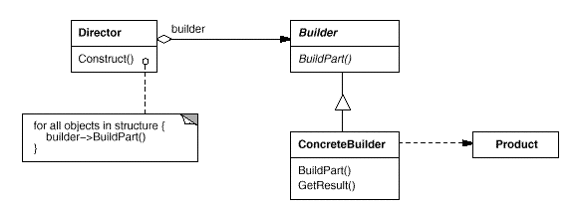
\includegraphics[width=\textwidth]{Builder_stru}
\subsection{Participants}
\begin{description}
    \item [Builder] Specifies an abstract interface for creating \textbf{parts
    of a Product object}
    \item[ConcreteBuilder]
        \begin{itemize}
        \item Construct and assembles parts of the product
        \item Defines and keeps track of the representation it creates.
        \item Provides an interface for \textbf{retrieving the product}
        \end{itemize}
    \item [Director] constructs an object using the Builder interface.
    \item [Product] Represents the complex object under construction.
    ConcreteBuilder builds the product's internal representation and defines teh
    process by which it's assembled.
\end{description}
\subsection{Collaborations}
\begin{enumerate}
\item The clients creates the Director and the Builder object.
\item Director notifies the builder whenever a part of the product should be
built.
\item Builder handles request and adds parts to the product.
\item The client retrieves the product from the builder
\end{enumerate}
\subsection{Consequence}
\begin{enumerate}
    \item Lets you vary a product's internal representation.
    \item It isolates code for construction and representation. The Builder improves
    modularity by encapsulating the way a complex object is constructed and
    represented.
    \item It gives you finer control over the construction process. It builds
    product step by step under the director's control.
\end{enumerate}
\subsection{Implementation}
Here are other implementation issues to consider:
\begin{enumerate}
    \item Assembly and construction interface. Builders construct their product
    step-by-step fashion.

    A key design issue concerns the model for the construction and assembly
    process.
    A model where the results of construction requests are simply appended to the
    product is usually sufficient. 

    But sometimes you might need access to parts of the product constructed
    earlier. In that case, the builder would return child nodes to the director,
    which then would pass them back to the builder to build the parent node.

    \item Why no abstract class for product? In the common case, the products
    produced by the concrete builders differ so greatly in their representation
    that there is little to gain from giving different products a common parent
    class. Because the client usually configures the director with the proper
    concrete builder, \emph{the client is in a position to know which concrete
    subclass of Builder is in use and can handle its products accordingly.}
    \item Empty methods as default in Builder.
\end{enumerate}
\subsection{Sample Code}
We'll define a variance of \verb|CreateMaze| member function that takes a
builder of class \verb|MazeBuiler| as an argument. 
\begin{verbatim}
class MazeBuilder {
public:
    virtual void BuildMaze() { }
    virtual void BuildRoom(int room) { }
    virtual void BuildDoor(int roomFrom, int roomTo) { }

    virtual Maze* GetMaze() {return 0; }
protected:
    MazeBuilder();
};
\end{verbatim}
This interface can create three things: 
\begin{enumerate}
\item The maze
\item Rooms with a particular room number
\item Doors between numbered rooms.
\end{enumerate}

All the maze-building operations of \verb|MazeBuilder| do nothing by default.

Given the \verb|MazeBuilder| interface, we can change the \verb|CreateMaze|
member function to take this builder as a parameter

\begin{verbatim}
Maze* MazeGame::CreateMaze (MazeBuilder& builder) {
//Build parts one by one
    builder.BuildMaze();

    builder.BuildRoom(1);
    builder.BuildRoom(2);
    builder.BuildDoor(1,2);

//Retrieve the product.
    return  builder.GetMaze();
}
\end{verbatim}

Like the other creational patterns, the Builder pattern encapsulates how objects
get created, in this case through the interface defined by MazeBuilder. That
means we can reuse MazeBuilder to build different kinds of mazes. Example:
\begin{verbatim}
Maze* MazeGame::CreateComplexMaze (MazeBuilder& builder) {
    builder.BuildRoom(1);
    // ...
    builder.BuildRoom(1001);

    return builder.GetMaze();
}
\end{verbatim}

Note that \verb|MazeBuilder| \textbf{does not create mazes itself}; its main
purpose is just to define an interface for creating mazes. It defines empty
implementations primarily for convenience. Subclass of \verb|MaeBuilder| do the
actual work:
\begin{verbatim}
class StandardMazeBuilder: public MazeBuilder {
public:
    StandardMazeBuilder();
    virtual void BuildMaze();
    virtual void BuildRoom(int);
    virtual void BuildDoor(int, int);

    virtual Maze* GetMaze();
private:
//CommonWall is a utility operation that determines the direction of the common
wall between two rooms.
    Direction CommonWall(Room*, Room*);
    Maze* _currentMaze;
};
StandardMazeBuilder::StandardMazeBuilder() {
    _currentMaze = 0
}

void StandardMazeBuilder::BuildMaze() {
    _currentMaze = 0;
}

Maze* StandardMazeBuilder::GetMaze() {
    return _currentMaze;
}

void StandardMazeBuilder::BuildRoom(int n) {
    if(!_currentMaze->RoomNo(n) {
        _currentMaze->AddRoom(room);

        room->SetSide(North, new Wall);
        room->SetSide(South, new Wall);
        room->SetSide(East, new Wall);
        room->SetSide(West, new Wall);
    }
}

void StandardMazeBuilder::BuildDoor (int n1, int n2) {
    Room* r1 = _currentMaze->RoomNo(n1);
    Room* r2 = _currentMaze->RoomNo(n2);
    Door* d = new Door(r1, r2);

    r1->SetSide(CommonWall(r1,r2), d);
    r2->SetSide(CommonWall(r2,r1), d);
}

//Clients can now use CreateMaze in conjunction with StandardMazeBuilder to
//create a maze:
Maze* maze;
MazeGame game;
StandardMazeBuilder builder;
game.CreateMaze(builder);
maze = builder.GetMaze();
\end{verbatim}

\subsection{Known Uses}
Common pattern Smalltalk-80:
\begin{itemize}
    \item The Parser class in the compiler subsystem is a Director that takes a
    ProgramNodeBuilder object as an argument. Parser provide syntactic construct
    and builder will build the parse tree.
    \item ClassBuilder is a builder that Classes use to create subclasses for
    themselves. Class is both the Director and the Product.
    \item ByteCodeStream is a builder that creates a compiled method as a byte
    array.
\end{itemize}

\section{Factory Method}
\subsection{Intent}
Define an interface for creating an object, but let subclasses decide which
class to instantiate.

Factory Method lets a class \textbf{defer instantiation to subclass}. Also know
as virtual constructor.

\subsection{Motivation}
Define and maintain relationships between objects.

Consider a framework for applications that can present multiple documents to the
user. Two abstraction:
\begin{itemize}
\item Classes Application
\item Document
\end{itemize}
Application class is responsible for managing Documents and will create as
required, when the user selects Open or New from a menu, for example.

Because the particular Document subclass to instantiate is
\textbf{application-specific}, he Application class \emph{can't predict the
subclass of Document to instantiate}

The application only knows \textbf{when} a new document should be created, not
\textbf{what kind} of Document to create.

Solution: Application subclasses redefine an abstract CreateDocument operation
on Application to return the appropriate Document subclass. We call
CreateDocument a \textbf{factory method} because it's responsible for
"manufacturing" an object.

\subsection{Applicability}
Use Factory Method pattern when:
\begin{itemize}
\item a class can't anticipate the class of objects it must create
\item A class wants its subclasses to specify the objects it creates.
\item Localize the knowledge of which helper subclass is delegate.
\end{itemize}
\subsection{Participants}
\begin{description}
\item [Product] defines the interface of the object the method creates.
\item [ConcreteProduct] implements the product interface
\item [Creator] declares factory method. May call factory method to create
Product.
\item [ConcreteCreator] Overrides the factory method.
\end{description}
\subsection{Consequence}
\begin{enumerate}
    \item Eliminate the need to bind application-specific classes into your code.
    \item Disadvantage: have to subclas the Creator class just to create a
    particular ConcreteProduct object.
    \item Provides hook for subclasses.
    \item Connects parallel class hierarchies.
\end{enumerate}
\section{Prototype}
\subsection{Intent}
Specify the kinds of objects to create using a prototypical instance, and create
new objects by copying this prototype.
\subsection{Motivation}
Build an editor for music scores by customizing a general framework for
graphical editors and adding new objects that represent notes, rests, etc. Let's
assume the framework provides an abstract graphic class for graphical
components, like notes and staves. The framework also predefine a GraphicTool
subclass for tools that create instances of graphical objects and add them to
the document.

But GraphicTool presents a problem: \emph{the class for notes and staves are specific
to our application, but the GraphicTool belongs to the framework}, GraphicTool
doesn't know how to create instances of our music classes to add to the score.
We could subclass GraphicTool for each kind of music object, but that would
produce lots of subclasses that differ only in the kind of music object they
instantiate.

The solution lies in making GraphicTool create a new Graphic by copying or
"cloning" an instance of a Graphic subclass. We call this instance a
\textbf{prototype} 

So in our music editor, each tool for creating a music object is an
\emph{instance of GraphicTool that's initialized with a different prototype},
Each GraphicTool instance will produce a music object by cloning its prototype
and adding the clone to the score. This can reduce the number of classes in the
system dramatically.

\subsection{Applicability}
\begin{itemize}
    \item A system should be independent of how its products are created.
    \item The class to instantiate are specified at run time.
    \item Avoid building a class hierarchy of factories that parallels the class
        hierarchy of products.
    \item When instances of a class can have one of only a few different
        combinations of state.
\end{itemize}
\subsection{Structure}
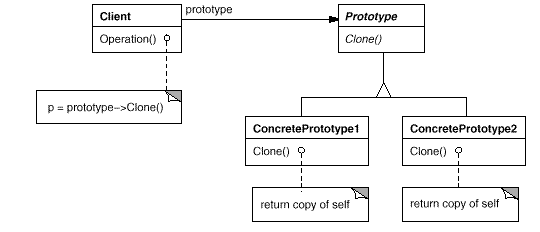
\includegraphics{Proto_stru}
\subsection{Participants}
\begin{description}
    \item [Prototype] declare an interface for cloning itself.
    \item [ConcretePrototype], implements an operation for cloning itself.
    \item [Client] Creates a new object by asking prototype to clone itself.
\end{description}
\subsection{Consequence}
\begin{enumerate}
    \item Adding and removing products at runtime.
    \item Specifying new objects by varying values. You effectively define new
        kinds of objects by instantiating existing classes and registering the
        instances as prototypes of client objects. This kind of design lets user
        \emph{define new "classes" without programming.}
    \item Specifying new objects by varying structure.
    \item Reduced subclassing
    \item Configuring an application with classes dynamically.
\end{enumerate}
\subsection{Implementation}
\begin{enumerate}
    \item Using a prototype manager. When the number of prototypes in a system
        isn't fixed, keep a registry of available prototypes. \emph{Clients
            won't manage prototypes themselves but will store and retrieve them
        from the registry.} A client will ask the registry for a prototype
        before cloning it. We call this registry a \textbf{prototype manager}
    \item Implementing the Clone operation.
    \item Initializing clones.
\end{enumerate}

\end{document}
